% Déclaration du type de document (report, book, paper, etc...)
\documentclass[a4paper]{paper} 
 
% Package pour avoir Latex en français
\usepackage[utf8]{inputenc}
\usepackage[francais]{babel}
 
% Quelques packages utiles
\usepackage{listings} % Pour afficher des listings de programmes
\usepackage{graphicx} % Pour afficher des figures
\usepackage{amsthm}   % Pour créer des théorèmes et des définitions
\usepackage{amsmath}
\usepackage{microtype} % Optical margins FTW

\lstset{language=MATLAB}



% Auteur
\author{
Mathieu Rouvinez \\
\texttt{mathieu.rouvinez@gmx.net}
\and
Antoine Albertelli \\
\texttt{antoine.albertelli@gmail.com}
\and
Florian Reinhard \\
\texttt{florian.reinhard@epfl.ch}
}
 
% Titre du document
\title{Equations de mouvement pour 3-omniwheels}

% Début du document
\begin{document}

\maketitle
% \tableofcontents
\section{Hypothèses}
\begin{itemize}
    \item Les roues sont situées aux sommets d'un triangle équilatéral avec 120\degre entre elles.
    \item Chaque roue peut avoir un rayon différent.
    \item Chaque roue peut se trouver à une distance différente du centre du triangle équilatéral.
    \item Le référentiel du robot se trouve au centre du triangle équilatéral.
\end{itemize}

\section{Cinématique directe}

\begin{figure}[h]
    \centering
    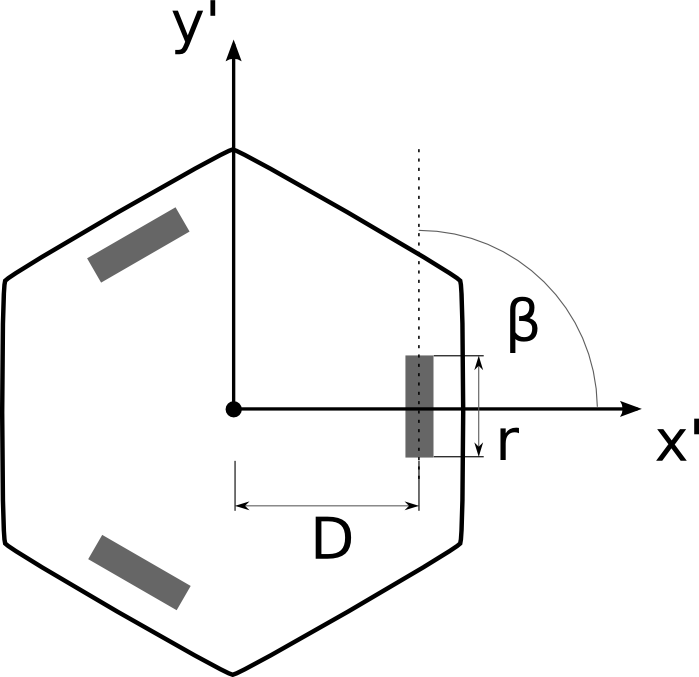
\includegraphics{holonomic_base.png}
    \caption{Les dimensions qui définissent la base holonome.}
    \label{fig:holonomic_base}
\end{figure}

\subsection{Translation}

\begin{equation}
    \omega_{i,t} = \frac{v}{r_i} \cdot \cos\left( \phi - \theta_V + \beta_i - \frac{\pi}{2} \right)
    \label{eqn:forward-translation}
\end{equation}

\begin{description}
    \item[$\omega_{i,t}$] Vitesse de rotation de la roue $i$ pour la translation de la base holonome.
    \item[$v$] Vitesse de déplacement du robot.
    \item[$\phi$] Angle absolu de l'orientation du robot.
    \item[$\theta_V$] Angle absolu de la direction de vitesse du robot.
    \item[$\beta_i$] Angle relatif au robot de l'orientation de la roue $i$.
    \item[$r_i$] Rayon de la roue $i$.
\end{description}
\subsubsection{Exemple en MATLAB}

\begin{lstlisting}
beta1 = 60*pi/180;
beta2 = 180*pi/180;
beta3 = 300*pi/180;
omega1_t = linear_speed_value / r1 * ...
           cos(heading-speed_angle+beta1-pi/2);
omega2_t = linear_speed_value / r2 * ...
           cos(heading-speed_angle+beta2-pi/2);
omega3_t = linear_speed_value / r3 * ...
           cos(heading-speed_angle+beta3-pi/2);
\end{lstlisting}

\subsection{Rotation}
\begin{equation}
    \omega_{i, r} = - \Omega \cdot \frac{D_i}{r_i}
    \label{eqn:forward-rotation}
\end{equation}

\begin{description}
    \item[$\omega_{i,r}$] Vitesse de rotation de la roue $i$ pour la rotation de la base holonome.
    \item[$\Omega$] Vitesse de rotation du robot sur lui même.
    \item[$D_i$] Distance entre le plan de rotation de la roue et le centre du robot.
    \item[$r_i$] Rayon de la roue $i$.
\end{description}
\subsubsection{Exemple en MATLAB}
\begin{lstlisting}
omega1_r = -angular_speed_value * D1 / r1;
omega2_r = -angular_speed_value * D2 / r2;
omega3_r = -angular_speed_value * D3 / r3;
\end{lstlisting}

\subsection{Combinaison}
En combinant \eqref{eqn:forward-translation} et \eqref{eqn:forward-rotation}, on obtient l'équation
pour un mouvement composé d'une translation et d'une rotation.
\begin{equation}
    \omega_i = \omega_{i,t} + \omega_{i,r}
    \label{eqn-forward-complete}
\end{equation}
\section{Cinématique inverse}
\subsection{Rotation}
\begin{equation}
    \theta_{R, t+1} = \theta_{R, t} - \frac{1}{steps} \frac{\sum\limits_{i=1}^3 steps_i \cdot r_i}{\sum\limits_{i=1}^3 r_i}
    \label{eqn:reverse-heading}
\end{equation}
\begin{description}
    \item[$\theta_R$] Orientation absolue du robot.
    \item[$steps$] Nombre de pas pour un tour de roue.
    \item[$steps_i$] Avancement de la roue $i$ en steps codeur.
    \item[$r_i$] Distance du plan de rotation de la roue $i$ au centre du robot.
\end{description}

\subsubsection{Exemple en MATLAB}
\begin{lstlisting}
heading = heading-(steps1*r1+steps2*r2+steps3*r3) ...
          /(D1+D2+D3)/steps_turn;
\end{lstlisting}

\subsection{Translation}
\begin{subequations}
    \begin{equation}
    \Delta_x = \frac{2}{3} \frac{1}{steps} \sum\limits_{i=1}^3 \cos \beta_i \cdot steps_i \cdot r_i 
    \end{equation}
    \begin{equation}
    \Delta_y = \frac{2}{3} \frac{1}{steps} \sum\limits_{i=1}^3 \sin \beta_i \cdot steps_i \cdot r_i 
    \end{equation}

    \label{eqn:reverse-translation}
\end{subequations}
\begin{description}
    \item[$\Delta_x$] Déplacement du robot selon l'axe X, dans son prore référentiel.
    \item[$\Delta_y$] Déplacement du robot selon l'axe Y, dans son prore référentiel.
    \item[$steps$] Nombre de pas pour un tour de roue.
    \item[$steps_i$] Avancement de la roue $i$ en steps codeur.
    \item[$\beta_i$] Angle relatif au robot de l'orientation de la roue $i$.
    \item[$r_i$] Rayon de la roue $i$.
\end{description}


\subsubsection{Exemple en MATLAB}
\begin{lstlisting}
mov_x = cos(beta1)*steps1*r1/steps_turn
      + cos(beta2)*steps2*r2/steps_turn
      + cos(beta3)*steps3*r3/steps_turn;
mov_y = sin(beta1)*steps1*r1/steps_turn
      + sin(beta2)*steps2*r2/steps_turn
      + sin(beta3)*steps3*r3/steps_turn;

mov_x = mov_x * 2/3;
mov_y = mov_y * 2/3;
\end{lstlisting}

\subsection{Conversion en coordonnées table}
Pour appliquer l'équation \eqref{eqn:reverse-translation}, il faut d'abord appliquer
la matrice de rotation du robot à $\Delta_x$ et $\Delta_y$:

\begin{subequations}
    \begin{equation}
        X = X + \cos \left( \theta_R - \frac{\pi}{2} \right) \cdot \Delta_x - \sin \left( \theta_R - \frac{\pi}{2} \right) \cdot \Delta_y
    \end{equation}
    \begin{equation} 
        Y = Y + \sin \left( \theta_R - \frac{\pi}{2} \right) \cdot \Delta_x + \cos \left( \theta_R - \frac{\pi}{2} \right) \cdot \Delta_y
    \end{equation} 
    \label{eqn:coordinate-transform}
\end{subequations}

\subsubsection{Exemple en MATLAB}
\begin{lstlisting}
pos_x = pos_x + cos(heading-pi/2)*mov_x - ...
        sin(heading-pi/2)*mov_y;
pos_y = pos_y + sin(heading-pi/2)*mov_x + ...
        cos(heading-pi/2)*mov_y;
\end{lstlisting}


\section{Intégration d'un IMU}

\subsection{\emph{Kalman Filter}}

\subsubsection{L'algorithme}

Control update:
\begin{equation}
    \bar{\mu}_t = g \left(u, \mu_{t-1} \right) 
\end{equation}

\begin{equation}
    \bar{\Sigma}_t = G_t \Sigma_{t-1} G_t^T + R_t
\end{equation}

Measurement update:
\begin{equation}
    K_t = \bar{\Sigma}_t H_t^T \left( H_t \bar{\Sigma}_t H_t^T + Q_t \right) ^{-1}
\end{equation}

\begin{equation}
    \mu_t = \bar{\mu}_t + K_t \left( z_t - h \left( \bar{\mu}_t \right) \right)
\end{equation}

\begin{equation}
    \Sigma_t = \left( I - K_t H_t \right) \bar{\Sigma}_t
\end{equation}

C'est l'algorithme d'un \emph{extended kalman filter} pour un \emph{control} et un
\emph{measurement} au même temps $ t $, mais il est aussi possible d'appliquer un
\emph{control update} sur un \emph{state belief} $ \bar{\mu}_{t-1} $, s'il y avait
pas encore un \emph{measurement}. Il est aussi possible d'avoir plusieurs,
différents \emph{measurements} et les intégrer avec la même formule.

Si l'erreur reel du \emph{control} et du \emph{measurement} est bien dans la
variation prévue ($ R_t $ et $ Q_t $), un \emph{measurement} normalement
diminue la variation du \emph{state}, qui s'accumule par juste appliquer
des \emph{controls}.

\subsubsection{Le cas d'un robot holonome}

\begin{figure}[h]
    \centering
    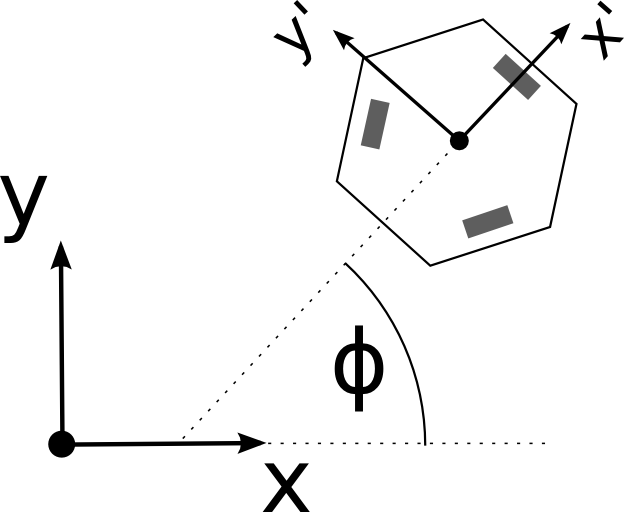
\includegraphics{coordinate_system.png}
    \caption{La définition du système des coordonnées local et global.}
    \label{fig:coordinate_system}
\end{figure}

\paragraph{Kalman state}

Le \emph{Kalman state} est représente par un vecteur, qui consiste dans ce cas des
coordonnées $x$ et $y$, l'orientation $\phi$ et leur dérivées correspondantes.

\begin{equation}
    \mu_t =
    \left( \begin{array}{c}
        x \\
        y \\
        \phi \\
        \dot{x} \\
        \dot{y} \\
        \dot{\phi} \\
    \end{array} \right)
    \label{State}
\end{equation}

\paragraph{Kalman control}

Un \emph{Kalman control} contient des informations imprévisibles, qui s'effectuent
sur le \emph{state} et qui est préférablement la dérivée du plus grand ordre dans
le système.
Les mesures de la \emph{IMU} sont exactement ça.

\begin{equation}
    u_t =
    \left( \begin{array}{c}
        a_x \\
        a_y \\
        \Omega_z \\
    \end{array} \right)
    \label{Control}
\end{equation}

\paragraph{Kalman measurement}

Une mesure \emph{Kalman} est un input, qui ce laisse prévoir à partir du \emph{state}
actuel.
Comme par exemple la vitesse de rotation des roues $ \omega_i $ ou une
mesure absolue de la position (balises).

\begin{equation}
    z_t =
    \left( \begin{array}{c}
        \omega_1 \\
        \omega_2 \\
        \omega_3 \\
    \end{array} \right)
    \label{Measurement}
\end{equation}

\paragraph{Fonction de transfert de control à state}

Une fonction $ g \left(u, \mu \right) $ calcule un \emph{state belief}
$ \bar{\mu} $ à partir du \emph{state} actuel et du \emph{control}.

\begin{equation}
    g \left(u, \mu \right) =
    \left( \begin{array}{l}
        x + \Delta t \cdot \dot{x} \\
        y + \Delta t \cdot \dot{y} \\
        \phi + \Delta t \cdot \dot{\phi} \\
        \dot{x} + \Delta t \cdot (cos(\phi) \cdot a_x + sin(\phi) \cdot a_y) \\
        \dot{y} + \Delta t \cdot (sin(\phi) \cdot a_x + cos(\phi) \cdot a_y) \\
        \Omega_z \\
    \end{array} \right)
    \label{g}
\end{equation}

\paragraph{G}

Parce que un filtre \emph{Kalman} fonctionne seulement avec des fonctions de transfert
linéaires, on prend l'expansion Taylor du premier degré. Pour cela on a besoin
du jacobien de $ g(u, \mu) $.

\begin{equation}
    G \left(u, \mu \right) =
    \left( \begin{array}{cccccc}
        1 & 0 & 0 & \Delta t & 0 & 0\\
        0 & 1 & 0 & 0 & \Delta t & 0\\
        0 & 0 & 1 & 0 & 0 & \Delta t\\
        0 & 0 & \Delta t \cdot (-sin(\phi) \cdot a_x + cos(\phi) \cdot a_y) & 1 & 0 & 0 \\
        0 & 0 & \Delta t \cdot ( cos(\phi) \cdot a_x - sin(\phi) \cdot a_y) & 0 & 1 & 0 \\
        0 & 0 & 0 & 0 & 0 & 0 \\
    \end{array} \right)
    \label{G}
\end{equation}

\paragraph{Fonction de transfert du state belief à measurement}

La fonction qui prévoit la vitesse de rotation des roues à partir du \emph{state}.

\begin{equation}
    h \left(u, \bar{\mu}\right) =
    \left( \begin{array}{l}
        \frac{\sqrt{\dot{x}^2 + \dot{y}^2}}{r_1} \cdot \cos \left( \phi - \tan^{-1} \left(\frac{\dot{y}}{\dot{x}}\right) + \beta_1 - \frac{\pi}{2} \right)
            - \dot{\phi} \cdot \frac{D_1}{r_1} \\
        \frac{\sqrt{\dot{x}^2 + \dot{y}^2}}{r_2} \cdot \cos \left( \phi - \tan^{-1} \left(\frac{\dot{y}}{\dot{x}}\right) + \beta_2 - \frac{\pi}{2} \right)
            - \dot{\phi} \cdot \frac{D_2}{r_2} \\
        \frac{\sqrt{\dot{x}^2 + \dot{y}^2}}{r_3} \cdot \cos \left( \phi - \tan^{-1} \left(\frac{\dot{y}}{\dot{x}}\right) + \beta_3 - \frac{\pi}{2} \right)
            - \dot{\phi} \cdot \frac{D_3}{r_3} \\
    \end{array} \right)
    \label{h}
\end{equation}
Il faut utiliser \texttt{atan2()} pour $ tan^{-1} \left(\frac{\dot{y}}{\dot{x}} \right) $.


\paragraph{H}

Le jacobien de $ h\left(u, \bar{\mu}\right) $.

\begin{equation}
    H\left(\bar{\mu}\right) =
    \left( \begin{array}{cccccc}
        \frac{\partial h_1\left(\bar{\mu}\right)}{\partial x} & \frac{\partial h_1(\bar{\mu})}{\partial y} & \frac{\partial h_1(\bar{\mu})}{\partial \phi} &
        \frac{\partial h_1\left(\bar{\mu}\right)}{\partial \dot{x}} & \frac{\partial h_1(\bar{\mu})}{\partial \dot{y}} & \frac{\partial h_1(\bar{\mu})}{\partial \dot{\phi}}\\
        \frac{\partial h_2\left(\bar{\mu}\right)}{\partial x} & \frac{\partial h_2(\bar{\mu})}{\partial y} & \frac{\partial h_2(\bar{\mu})}{\partial \phi} &
        \frac{\partial h_2\left(\bar{\mu}\right)}{\partial \dot{x}} & \frac{\partial h_2(\bar{\mu})}{\partial \dot{y}} & \frac{\partial h_2(\bar{\mu})}{\partial \dot{\phi}}\\
        \frac{\partial h_3\left(\bar{\mu}\right)}{\partial x} & \frac{\partial h_3(\bar{\mu})}{\partial y} & \frac{\partial h_3(\bar{\mu})}{\partial \phi} &
        \frac{\partial h_3\left(\bar{\mu}\right)}{\partial \dot{x}} & \frac{\partial h_3(\bar{\mu})}{\partial \dot{y}} & \frac{\partial h_3(\bar{\mu})}{\partial \dot{\phi}}\\
    \end{array} \right)
    \label{}
\end{equation}

On pose:

\[ \begin{array}{ccc}
    v = \sqrt{\dot{x}^2 + \dot{y}^2}, &
    \frac{\partial v}{\partial \dot{x}} = \frac{\dot{x}}{v}, &
    \frac{\partial v}{\partial \dot{y}} = \frac{\dot{y}}{v} \\
\end{array} \]

\[ \begin{array}{ccc}
    \theta = \tan^{-1}\left( \frac{\dot{y}}{\dot{x}} \right), &
    \frac{\partial \theta}{\partial \dot{x}} = - \frac{\dot{y}}{v^2}, &
    \frac{\partial \theta}{\partial \dot{y}} = \frac{\dot{x}}{v^2} \\
\end{array} \]

\[ \Psi_i = \phi - \theta + \beta_i - \frac{\pi}{2} \]

Alors,

\begin{equation}
    \begin{array}{l}
        \frac{\partial h_i\left(\bar{\mu}\right)}{\partial x} = 0 \\
        \frac{\partial h_i\left(\bar{\mu}\right)}{\partial y} = 0 \\
        \frac{\partial h_i\left(\bar{\mu}\right)}{\partial \phi} = - \frac{v}{r_i} \cdot \sin \left( \Psi_i \right) \\
        \frac{\partial h_i\left(\bar{\mu}\right)}{\partial \dot{x}} = \frac{\dot{x}}{r_i \cdot v} \cdot \cos \left( \Psi_i \right)
            - \frac{\dot{y}}{r_i \cdot v} \sin \left( \Psi_i \right) \\
        \frac{\partial h_i\left(\bar{\mu}\right)}{\partial \dot{y}} = \frac{\dot{y}}{r_i \cdot v} \cdot \cos \left( \Psi_i \right)
            + \frac{\dot{x}}{r_i \cdot v} \sin \left( \Psi_i \right)\\
        \frac{\partial h_i\left(\bar{\mu}\right)}{\partial \dot{\phi}} = - \frac{D_i}{r_i}\\
    \end{array}
\end{equation}

\paragraph{Covariance du \emph{control}}
\begin{equation}
    R =
    \left( \begin{array}{ccc}
        S_{a_x} & 0 & 0 \\
        0 & S_{a_y} & 0 \\
        0 & 0 & S_{\Omega_z} \\
    \end{array} \right)
\end{equation}

\paragraph{Covariance du \emph{measurement}}
\begin{equation}
    Q =
    \left( \begin{array}{ccc}
        S_{\omega_1} & 0 & 0 \\
        0 & S_{\omega_2} & 0 \\
        0 & 0 & S_{\omega_3} \\
    \end{array} \right)
\end{equation}

\paragraph{Covariance initiale du \emph{state}}
\begin{equation}
    \Sigma_0 =
    \left( \begin{array}{cccccc}
        S_{x_0} & 0 & 0 & 0 & 0 & 0 \\
        0 & S_{y_0} & 0 & 0 & 0 & 0 \\
        0 & 0 & S_{\phi_0} & 0 & 0 & 0 \\
        0 & 0 & 0 & 0 & 0 & 0 \\
        0 & 0 & 0 & 0 & 0 & 0 \\
        0 & 0 & 0 & 0 & 0 & 0 \\
    \end{array} \right)
\end{equation}

Il faut trouver la precision avec laquelle on arrive à positionner le robot au
début du match. On peut dire que la variation initiale de la vitesse est bien
égale à zéro.


\end{document}
